\documentclass[a4paper]{book}
\usepackage{a4wide}
\usepackage{makeidx}
\usepackage{graphicx}
\usepackage{multicol}
\usepackage{float}
\usepackage{listings}
\usepackage{color}
\usepackage{textcomp}
\usepackage{alltt}
\usepackage{times}
\usepackage{ifpdf}
\ifpdf
\usepackage[pdftex,
            pagebackref=true,
            colorlinks=true,
            linkcolor=blue,
            unicode
           ]{hyperref}
\else
\usepackage[ps2pdf,
            pagebackref=true,
            colorlinks=true,
            linkcolor=blue,
            unicode
           ]{hyperref}
\usepackage{pspicture}
\fi
\usepackage[utf8]{inputenc}
\usepackage{doxygen}
\lstset{language=C++,inputencoding=utf8,basicstyle=\footnotesize,breaklines=true,breakatwhitespace=true,tabsize=8,numbers=left }
\makeindex
\setcounter{tocdepth}{3}
\renewcommand{\footrulewidth}{0.4pt}
\begin{document}
\hypersetup{pageanchor=false}
\begin{titlepage}
\vspace*{7cm}
\begin{center}
{\Large dsjm }\\
\vspace*{1cm}
{\large Generated by Doxygen 1.6.1}\\
\vspace*{0.5cm}
{\small Thu Oct 6 10:58:45 2016}\\
\end{center}
\end{titlepage}
\clearemptydoublepage
\pagenumbering{roman}
\tableofcontents
\clearemptydoublepage
\pagenumbering{arabic}
\hypersetup{pageanchor=true}
\chapter{Todo List}
\label{todo}
\hypertarget{todo}{}
\label{todo__todo000002}
\hypertarget{todo__todo000002}{}
 
\begin{DoxyDescription}
\item[Class \hyperlink{classMatrix}{Matrix} ]
\end{DoxyDescription}
\chapter{Class Index}
\section{Class Hierarchy}
This inheritance list is sorted roughly, but not completely, alphabetically:\begin{DoxyCompactList}
\item \contentsline{section}{BucketPQ$<$ MinMaxQueue $>$}{\pageref{classBucketPQ}}{}
\item \contentsline{section}{Configuration}{\pageref{classConfiguration}}{}
\item \contentsline{section}{FD}{\pageref{classFD}}{}
\item \contentsline{section}{IRowColumnDS}{\pageref{classIRowColumnDS}}{}
\begin{DoxyCompactList}
\item \contentsline{section}{IMatrix}{\pageref{classIMatrix}}{}
\begin{DoxyCompactList}
\item \contentsline{section}{Matrix}{\pageref{classMatrix}}{}
\begin{DoxyCompactList}
\item \contentsline{section}{Eye}{\pageref{classEye}}{}
\end{DoxyCompactList}
\end{DoxyCompactList}
\end{DoxyCompactList}
\item \contentsline{section}{ltint}{\pageref{structltint}}{}
\item \contentsline{section}{DSJM::MemoryError}{\pageref{classDSJM_1_1MemoryError}}{}
\item \contentsline{section}{NNZTag}{\pageref{classNNZTag}}{}
\item \contentsline{section}{Result}{\pageref{classResult}}{}
\item \contentsline{section}{RLF}{\pageref{classRLF}}{}
\item \contentsline{section}{RunningTimeInfo}{\pageref{classRunningTimeInfo}}{}
\item \contentsline{section}{StructuredJacobian}{\pageref{classStructuredJacobian}}{}
\item \contentsline{section}{ColPack::Timer}{\pageref{classColPack_1_1Timer}}{}
\end{DoxyCompactList}

\chapter{Class Index}
\section{Class List}
Here are the classes, structs, unions and interfaces with brief descriptions:\begin{DoxyCompactList}
\item\contentsline{section}{\hyperlink{classBucketPQ}{BucketPQ$<$ MinMaxQueue $>$} }{\pageref{classBucketPQ}}{}
\item\contentsline{section}{\hyperlink{classConfiguration}{Configuration} }{\pageref{classConfiguration}}{}
\item\contentsline{section}{\hyperlink{classEye}{Eye} }{\pageref{classEye}}{}
\item\contentsline{section}{\hyperlink{classFD}{FD} }{\pageref{classFD}}{}
\item\contentsline{section}{\hyperlink{classIMatrix}{IMatrix} }{\pageref{classIMatrix}}{}
\item\contentsline{section}{\hyperlink{classIRowColumnDS}{IRowColumnDS} }{\pageref{classIRowColumnDS}}{}
\item\contentsline{section}{\hyperlink{structltint}{ltint} }{\pageref{structltint}}{}
\item\contentsline{section}{\hyperlink{classMatrix}{Matrix} }{\pageref{classMatrix}}{}
\item\contentsline{section}{\hyperlink{classDSJM_1_1MemoryError}{DSJM::MemoryError} }{\pageref{classDSJM_1_1MemoryError}}{}
\item\contentsline{section}{\hyperlink{classNNZTag}{NNZTag} }{\pageref{classNNZTag}}{}
\item\contentsline{section}{\hyperlink{classResult}{Result} }{\pageref{classResult}}{}
\item\contentsline{section}{\hyperlink{classRLF}{RLF} }{\pageref{classRLF}}{}
\item\contentsline{section}{\hyperlink{classRunningTimeInfo}{RunningTimeInfo} }{\pageref{classRunningTimeInfo}}{}
\item\contentsline{section}{\hyperlink{classStructuredJacobian}{StructuredJacobian} }{\pageref{classStructuredJacobian}}{}
\item\contentsline{section}{\hyperlink{classColPack_1_1Timer}{ColPack::Timer} (Class \hyperlink{classColPack_1_1Timer}{Timer} in \hyperlink{}{group4} )}{\pageref{classColPack_1_1Timer}}{}
\end{DoxyCompactList}

\chapter{Class Documentation}
\hypertarget{classBucketPQ}{
\section{BucketPQ$<$ MinMaxQueue $>$ Class Template Reference}
\label{classBucketPQ}\index{BucketPQ@{BucketPQ}}
}
\subsection*{Public Member Functions}
\begin{DoxyCompactItemize}
\item 
\hypertarget{classBucketPQ_a9f9ee7403058a116f4cc71265a24a6ec}{
{\bfseries BucketPQ} (int \_\-maxBucket, int \_\-numberOfItems)}
\label{classBucketPQ_a9f9ee7403058a116f4cc71265a24a6ec}

\item 
\hypertarget{classBucketPQ_a26a0a7623213a531dc485b479788bbd0}{
bool {\bfseries empty} () const }
\label{classBucketPQ_a26a0a7623213a531dc485b479788bbd0}

\item 
\hypertarget{classBucketPQ_a9a6f9fb1dc309b9abacbc846bb07ab9e}{
void {\bfseries insert} (Index vertex\_\-id, Priority priority)}
\label{classBucketPQ_a9a6f9fb1dc309b9abacbc846bb07ab9e}

\item 
\hypertarget{classBucketPQ_a3dde89127ed03fc51868b7d2aed90558}{
Item {\bfseries top} ()}
\label{classBucketPQ_a3dde89127ed03fc51868b7d2aed90558}

\item 
\hypertarget{classBucketPQ_abae85af7fccf22c3cc5448321385d2a4}{
void {\bfseries pop} ()}
\label{classBucketPQ_abae85af7fccf22c3cc5448321385d2a4}

\item 
\hypertarget{classBucketPQ_af12cf8b307eaf681b42f1d9845ba303f}{
Item {\bfseries get} (Index vertex\_\-id)}
\label{classBucketPQ_af12cf8b307eaf681b42f1d9845ba303f}

\item 
\hypertarget{classBucketPQ_a8112720b754173aefa8dc7bc60c6cb8a}{
void {\bfseries increase} (Index vertex\_\-id)}
\label{classBucketPQ_a8112720b754173aefa8dc7bc60c6cb8a}

\item 
\hypertarget{classBucketPQ_a2a83c56c6ab339b02595e29a8618ac1d}{
void {\bfseries decrease} (Index vertex\_\-id)}
\label{classBucketPQ_a2a83c56c6ab339b02595e29a8618ac1d}

\item 
\hypertarget{classBucketPQ_a901b7e69550fb03b4720a6ffc81110e2}{
void {\bfseries change} (Index vertex\_\-id, Priority priority)}
\label{classBucketPQ_a901b7e69550fb03b4720a6ffc81110e2}

\item 
\hypertarget{classBucketPQ_ae3cb097d11027f3e8277508dcfcf9a67}{
void {\bfseries remove} (Index vertex\_\-id)}
\label{classBucketPQ_ae3cb097d11027f3e8277508dcfcf9a67}

\item 
\hypertarget{classBucketPQ_af468d18437d36b4afc634c53f34b05fc}{
void {\bfseries make\_\-empty} ()}
\label{classBucketPQ_af468d18437d36b4afc634c53f34b05fc}

\item 
\hypertarget{classBucketPQ_a1eabfcc3affee86738816d259ebac587}{
Item {\bfseries betterTop} (int jp, const int maxlst, const int $\ast$ndeg)}
\label{classBucketPQ_a1eabfcc3affee86738816d259ebac587}

\end{DoxyCompactItemize}
\subsubsection*{template$<$typename MinMaxQueue$>$ class BucketPQ$<$ MinMaxQueue $>$}



The documentation for this class was generated from the following file:\begin{DoxyCompactItemize}
\item 
src/BucketPQ.hh\end{DoxyCompactItemize}

\hypertarget{classConfiguration}{
\section{Configuration Class Reference}
\label{classConfiguration}\index{Configuration@{Configuration}}
}
\subsection*{Public Member Functions}
\begin{DoxyCompactItemize}
\item 
\hyperlink{classConfiguration_a779947337bf652f0e773cb29f37f14ba}{Configuration} ()
\item 
virtual \hyperlink{classConfiguration_a0dd0fa189e239f4c9a036303f641441e}{$\sim$Configuration} ()
\end{DoxyCompactItemize}
\subsection*{Public Attributes}
\begin{DoxyCompactItemize}
\item 
\hypertarget{classConfiguration_a4c365cfe69250a8be96bcfa68313e222}{
CLI::ordering\_\-method {\bfseries oMethod}}
\label{classConfiguration_a4c365cfe69250a8be96bcfa68313e222}

\item 
\hypertarget{classConfiguration_a77b57b6ca01c5dff5fb3c5be944c5694}{
char $\ast$ {\bfseries inputfile}}
\label{classConfiguration_a77b57b6ca01c5dff5fb3c5be944c5694}

\item 
\hypertarget{classConfiguration_af6196c9d494debc50be608034a9b6336}{
bool {\bfseries statistics\_\-only}}
\label{classConfiguration_af6196c9d494debc50be608034a9b6336}

\item 
\hypertarget{classConfiguration_ae33cbe063d4adfed682736be782c2414}{
bool {\bfseries is\_\-cseg}}
\label{classConfiguration_ae33cbe063d4adfed682736be782c2414}

\item 
\hypertarget{classConfiguration_a792087f451846a90de7b415ca4982074}{
char $\ast$ {\bfseries partitionFile}}
\label{classConfiguration_a792087f451846a90de7b415ca4982074}

\item 
\hypertarget{classConfiguration_ae8a1b7716a1f5f02fb98d00a4e6ff673}{
bool {\bfseries extend}}
\label{classConfiguration_ae8a1b7716a1f5f02fb98d00a4e6ff673}

\item 
\hypertarget{classConfiguration_a07922b8c75587f61e9ad5c5ab87d3485}{
bool {\bfseries verify}}
\label{classConfiguration_a07922b8c75587f61e9ad5c5ab87d3485}

\item 
\hypertarget{classConfiguration_a2af5f378338489bf4c12c211334bc77f}{
bool {\bfseries inputfile\_\-given}}
\label{classConfiguration_a2af5f378338489bf4c12c211334bc77f}

\item 
\hypertarget{classConfiguration_afb3c182aeea4f111cc335664bcb0532a}{
bool {\bfseries io\_\-at\_\-end}}
\label{classConfiguration_afb3c182aeea4f111cc335664bcb0532a}

\item 
\hypertarget{classConfiguration_a0349f61f85d781a3d776bef8bc19e4c2}{
string {\bfseries exeName}}
\label{classConfiguration_a0349f61f85d781a3d776bef8bc19e4c2}

\item 
\hypertarget{classConfiguration_ad9b3d3735ae57b036dcc841ebe11f23f}{
string {\bfseries commandLine}}
\label{classConfiguration_ad9b3d3735ae57b036dcc841ebe11f23f}

\item 
\hypertarget{classConfiguration_ae1c91512831b6c5fcdb67e1bb788b560}{
bool {\bfseries is\_\-symmetric}}
\label{classConfiguration_ae1c91512831b6c5fcdb67e1bb788b560}

\item 
\hypertarget{classConfiguration_a7efb05042deafcc6cdad146b4a5d15ef}{
bool {\bfseries is\_\-pattern}}
\label{classConfiguration_a7efb05042deafcc6cdad146b4a5d15ef}

\item 
\hypertarget{classConfiguration_a6a7146d171b8a44c03069d3ccb8b7e9d}{
bool {\bfseries is\_\-load\_\-each\_\-row\_\-as\_\-partition}}
\label{classConfiguration_a6a7146d171b8a44c03069d3ccb8b7e9d}

\item 
\hypertarget{classConfiguration_a9db655020ed3d2752a16daef0ccce66e}{
int {\bfseries M}}
\label{classConfiguration_a9db655020ed3d2752a16daef0ccce66e}

\item 
\hypertarget{classConfiguration_af6362e29173fb6b80ce82097abb879df}{
int {\bfseries N}}
\label{classConfiguration_af6362e29173fb6b80ce82097abb879df}

\item 
\hypertarget{classConfiguration_a145b6ac832c1ad733bc709f0a99f4c4c}{
int {\bfseries nz}}
\label{classConfiguration_a145b6ac832c1ad733bc709f0a99f4c4c}

\item 
\hypertarget{classConfiguration_a81b88410b064d6cf37224fd4c743abe9}{
int {\bfseries NZ}}
\label{classConfiguration_a81b88410b064d6cf37224fd4c743abe9}

\end{DoxyCompactItemize}


\subsection{Constructor \& Destructor Documentation}
\hypertarget{classConfiguration_a779947337bf652f0e773cb29f37f14ba}{
\index{Configuration@{Configuration}!Configuration@{Configuration}}
\index{Configuration@{Configuration}!Configuration@{Configuration}}
\subsubsection[{Configuration}]{\setlength{\rightskip}{0pt plus 5cm}Configuration::Configuration ()}}
\label{classConfiguration_a779947337bf652f0e773cb29f37f14ba}
: Constructor  Date: 05.08.2009 \hypertarget{classConfiguration_a0dd0fa189e239f4c9a036303f641441e}{
\index{Configuration@{Configuration}!$\sim$Configuration@{$\sim$Configuration}}
\index{$\sim$Configuration@{$\sim$Configuration}!Configuration@{Configuration}}
\subsubsection[{$\sim$Configuration}]{\setlength{\rightskip}{0pt plus 5cm}Configuration::$\sim$Configuration ()\hspace{0.3cm}{\ttfamily  \mbox{[}virtual\mbox{]}}}}
\label{classConfiguration_a0dd0fa189e239f4c9a036303f641441e}
: Desctructor  Date: 05.08.2009 

The documentation for this class was generated from the following files:\begin{DoxyCompactItemize}
\item 
src/Configuration.hh\item 
src/Configuration.cc\end{DoxyCompactItemize}

\hypertarget{classEye}{
\section{Eye Class Reference}
\label{classEye}\index{Eye@{Eye}}
}
Inheritance diagram for Eye::\begin{figure}[H]
\begin{center}
\leavevmode
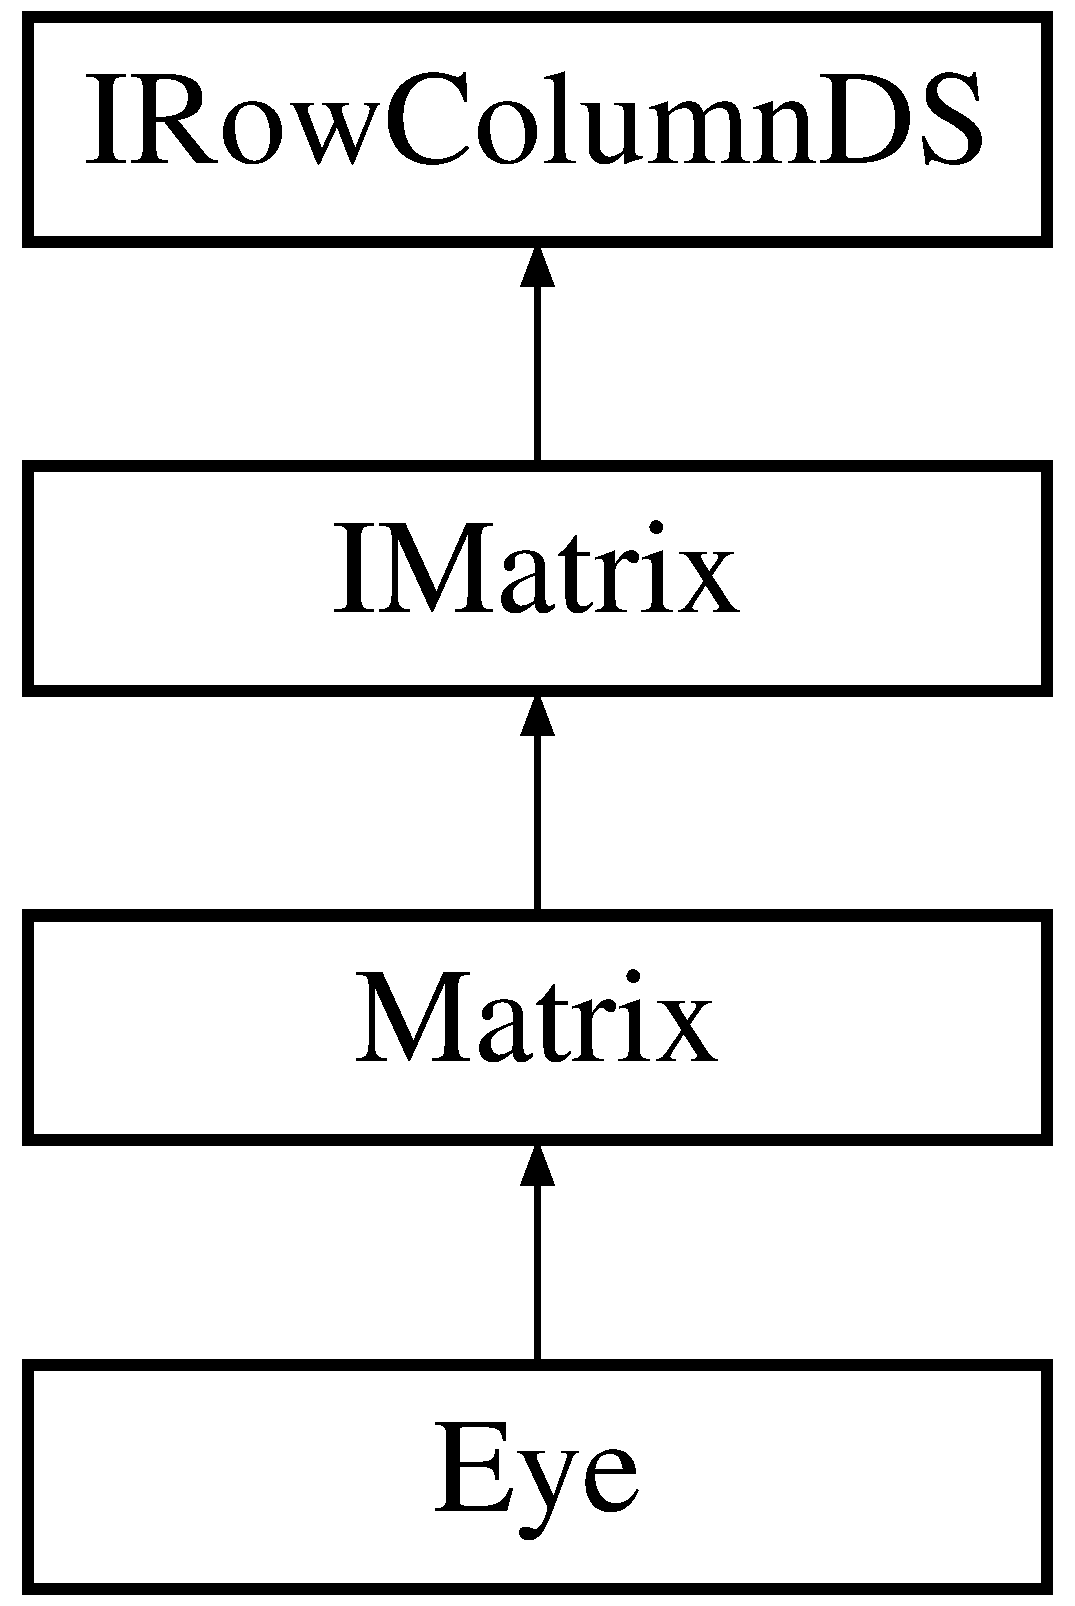
\includegraphics[height=4cm]{classEye}
\end{center}
\end{figure}
\subsection*{Public Member Functions}
\begin{DoxyCompactItemize}
\item 
\hypertarget{classEye_a30767316add2197e9f37971f0193d64a}{
{\bfseries Eye} (int n)}
\label{classEye_a30767316add2197e9f37971f0193d64a}

\end{DoxyCompactItemize}


The documentation for this class was generated from the following file:\begin{DoxyCompactItemize}
\item 
examples/Eye.hh\end{DoxyCompactItemize}

\hypertarget{classFD}{
\section{FD Class Reference}
\label{classFD}\index{FD@{FD}}
}
\subsection*{Static Public Member Functions}
\begin{DoxyCompactItemize}
\item 
\hypertarget{classFD_a47fa71e21563e15bbe74055507a6b9ae}{
{\footnotesize template$<$class Function , class SeedMatrix $>$ }\\static \hyperlink{classMatrix}{Matrix} $\ast$ {\bfseries finiteDifference} (Function f, const vector$<$ double $>$ \&x, SeedMatrix $\ast$seed)}
\label{classFD_a47fa71e21563e15bbe74055507a6b9ae}

\end{DoxyCompactItemize}


The documentation for this class was generated from the following file:\begin{DoxyCompactItemize}
\item 
examples/FD.hh\end{DoxyCompactItemize}

\hypertarget{classIMatrix}{
\section{IMatrix Class Reference}
\label{classIMatrix}\index{IMatrix@{IMatrix}}
}
Inheritance diagram for IMatrix::\begin{figure}[H]
\begin{center}
\leavevmode
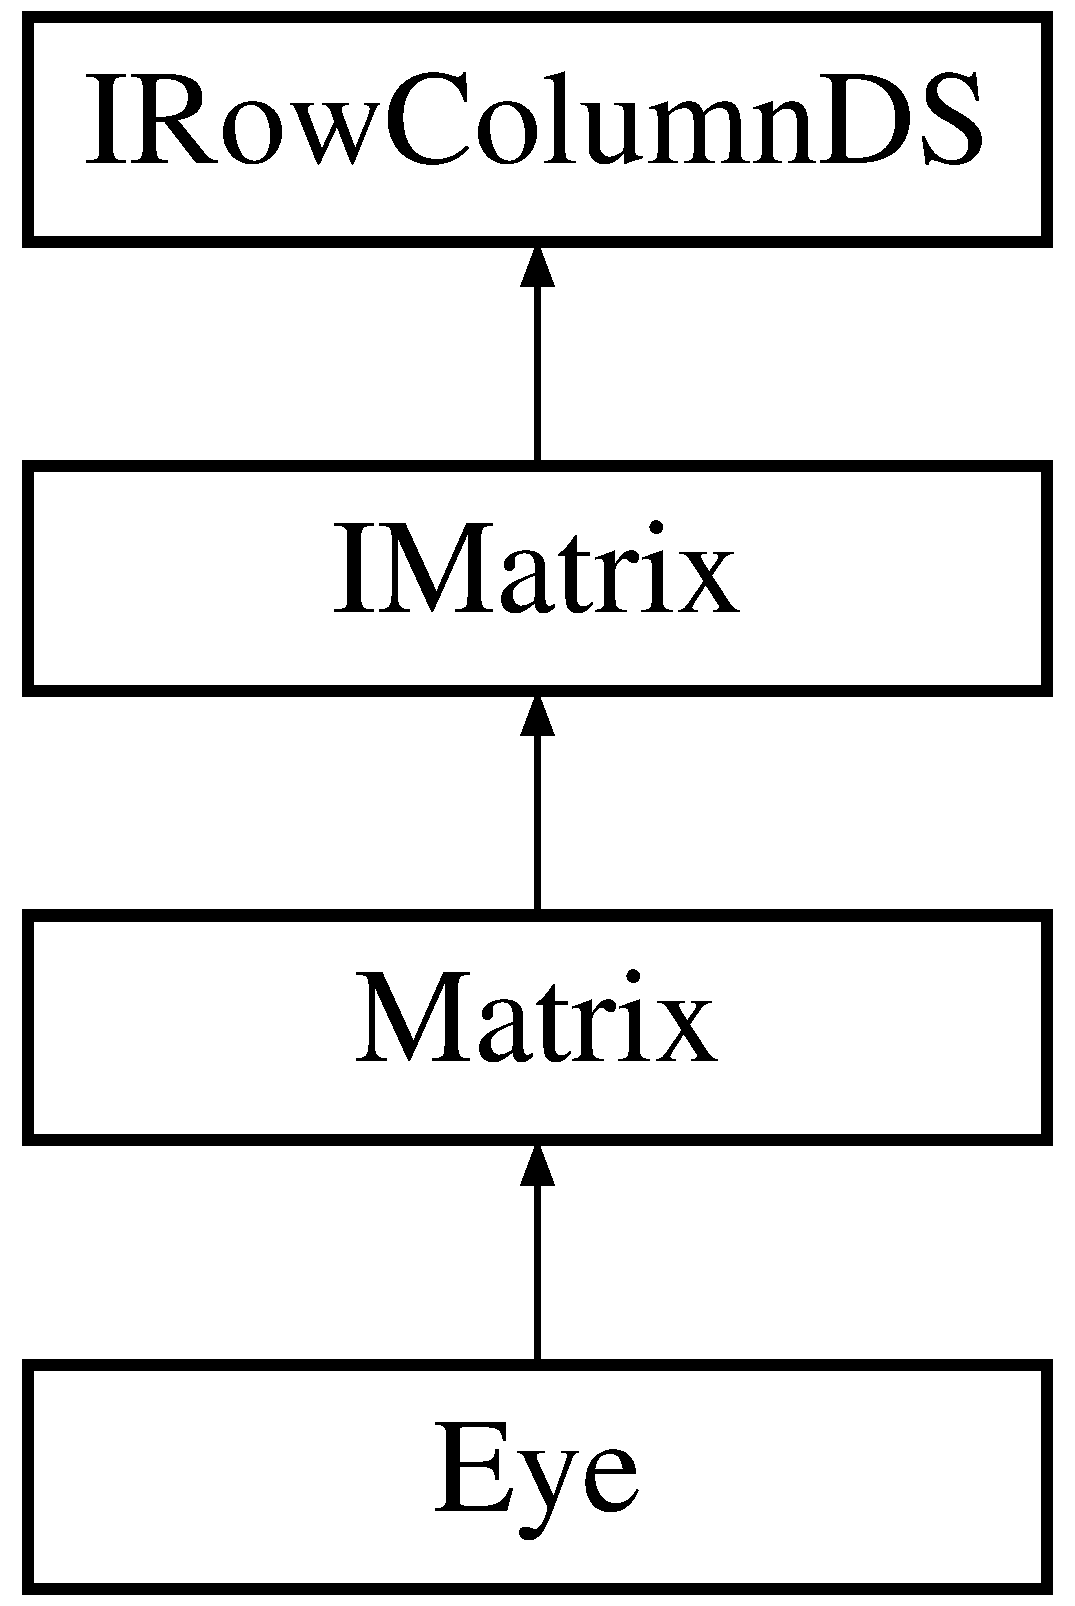
\includegraphics[height=4cm]{classIMatrix}
\end{center}
\end{figure}
\subsection*{Public Member Functions}
\begin{DoxyCompactItemize}
\item 
\hyperlink{classIMatrix_afe2001929e7328d988dc1d85c0d18c27}{IMatrix} (int M, int N, int nz, bool value)
\item 
virtual bool \hyperlink{classIMatrix_ad6d689b7a38120b6463f1965915f7163}{slo} (int $\ast$order)=0
\item 
virtual bool \hyperlink{classIMatrix_a8e0f3a1062786b6a20548e847de1109b}{ido} (int $\ast$order)=0
\item 
\hypertarget{classIMatrix_a3e7d104e9d2f662b59e59d84b60b1260}{
virtual bool {\bfseries lfo} (int $\ast$order)=0}
\label{classIMatrix_a3e7d104e9d2f662b59e59d84b60b1260}

\item 
\hypertarget{classIMatrix_adba40eab9af7ad22f2519493dc2cc50d}{
virtual bool {\bfseries computedegree} ()=0}
\label{classIMatrix_adba40eab9af7ad22f2519493dc2cc50d}

\item 
\hypertarget{classIMatrix_afa61e6e0a0baf59bd5c898ef759fc5f0}{
virtual int {\bfseries greedycolor} (int $\ast$list, int $\ast$ngrp)=0}
\label{classIMatrix_afa61e6e0a0baf59bd5c898ef759fc5f0}

\item 
\hypertarget{classIMatrix_a48855671733fe3f89e96f3c9a606d04f}{
virtual int {\bfseries rlf} (int $\ast$ngrp)=0}
\label{classIMatrix_a48855671733fe3f89e96f3c9a606d04f}

\item 
\hypertarget{classIMatrix_aa62c5ede68855fb7a3cf5332767b9699}{
void {\bfseries setVerify} (bool v)}
\label{classIMatrix_aa62c5ede68855fb7a3cf5332767b9699}

\item 
\hypertarget{classIMatrix_af112ae04ef11c8e780b9e11196442eb0}{
bool {\bfseries getVerify} ()}
\label{classIMatrix_af112ae04ef11c8e780b9e11196442eb0}

\item 
\hypertarget{classIMatrix_ac866b3b6ae6ed3802207617cbe083636}{
void {\bfseries buildPriorityQueue} (int n, int $\ast$ndeg, int $\ast$head, int $\ast$next, int $\ast$previous)}
\label{classIMatrix_ac866b3b6ae6ed3802207617cbe083636}

\item 
void \hyperlink{classIMatrix_adef00da9cba0f17ec0d64d688a3ebc58}{deleteColumn} (int $\ast$head, int $\ast$next, int $\ast$previous, int numdeg, int jcol)
\item 
void \hyperlink{classIMatrix_adfe1c1b95399cadb8d07a17d10ea6118}{addColumn} (int $\ast$head, int $\ast$next, int $\ast$previous, int numdeg, int jcol)
\item 
\hypertarget{classIMatrix_a43dbfcf605af6de605db7c5c95cecca4}{
void {\bfseries initializeDegreesToUVertices} (int n, int $\ast$tag, int $\ast$u\_\-head, int $\ast$u\_\-next, int $\ast$u\_\-previous, int $\ast$u\_\-list, bool $\ast$f\_\-added, int $\ast$f\_\-tag)}
\label{classIMatrix_a43dbfcf605af6de605db7c5c95cecca4}

\end{DoxyCompactItemize}
\subsection*{Protected Attributes}
\begin{DoxyCompactItemize}
\item 
\hypertarget{classIMatrix_a131c3e77ce7a03f2655a633b147c07f9}{
bool {\bfseries shouldVerify}}
\label{classIMatrix_a131c3e77ce7a03f2655a633b147c07f9}

\item 
\hypertarget{classIMatrix_a64cd0699662ea81465c3b356e84cceab}{
int {\bfseries maxdeg}}
\label{classIMatrix_a64cd0699662ea81465c3b356e84cceab}

\end{DoxyCompactItemize}


\subsection{Constructor \& Destructor Documentation}
\hypertarget{classIMatrix_afe2001929e7328d988dc1d85c0d18c27}{
\index{IMatrix@{IMatrix}!IMatrix@{IMatrix}}
\index{IMatrix@{IMatrix}!IMatrix@{IMatrix}}
\subsubsection[{IMatrix}]{\setlength{\rightskip}{0pt plus 5cm}IMatrix::IMatrix (int {\em M}, \/  int {\em N}, \/  int {\em nz}, \/  bool {\em value})}}
\label{classIMatrix_afe2001929e7328d988dc1d85c0d18c27}
: This functions  Date: 20.06.2009 

\subsection{Member Function Documentation}
\hypertarget{classIMatrix_adfe1c1b95399cadb8d07a17d10ea6118}{
\index{IMatrix@{IMatrix}!addColumn@{addColumn}}
\index{addColumn@{addColumn}!IMatrix@{IMatrix}}
\subsubsection[{addColumn}]{\setlength{\rightskip}{0pt plus 5cm}void IMatrix::addColumn (int $\ast$ {\em head}, \/  int $\ast$ {\em next}, \/  int $\ast$ {\em previous}, \/  int {\em numdeg}, \/  int {\em jcol})}}
\label{classIMatrix_adfe1c1b95399cadb8d07a17d10ea6118}
Constant Operation \hypertarget{classIMatrix_adef00da9cba0f17ec0d64d688a3ebc58}{
\index{IMatrix@{IMatrix}!deleteColumn@{deleteColumn}}
\index{deleteColumn@{deleteColumn}!IMatrix@{IMatrix}}
\subsubsection[{deleteColumn}]{\setlength{\rightskip}{0pt plus 5cm}void IMatrix::deleteColumn (int $\ast$ {\em head}, \/  int $\ast$ {\em next}, \/  int $\ast$ {\em previous}, \/  int {\em numdeg}, \/  int {\em jcol})}}
\label{classIMatrix_adef00da9cba0f17ec0d64d688a3ebc58}
Constant Operation \hypertarget{classIMatrix_a8e0f3a1062786b6a20548e847de1109b}{
\index{IMatrix@{IMatrix}!ido@{ido}}
\index{ido@{ido}!IMatrix@{IMatrix}}
\subsubsection[{ido}]{\setlength{\rightskip}{0pt plus 5cm}virtual bool IMatrix::ido (int $\ast$ {\em order})\hspace{0.3cm}{\ttfamily  \mbox{[}pure virtual\mbox{]}}}}
\label{classIMatrix_a8e0f3a1062786b6a20548e847de1109b}
Method \hyperlink{classIMatrix_a8e0f3a1062786b6a20548e847de1109b}{ido()} 

Implemented in \hyperlink{classMatrix_ab9bef57c1115e601cdeb493ecb381b82}{Matrix}.\hypertarget{classIMatrix_ad6d689b7a38120b6463f1965915f7163}{
\index{IMatrix@{IMatrix}!slo@{slo}}
\index{slo@{slo}!IMatrix@{IMatrix}}
\subsubsection[{slo}]{\setlength{\rightskip}{0pt plus 5cm}virtual bool IMatrix::slo (int $\ast$ {\em order})\hspace{0.3cm}{\ttfamily  \mbox{[}pure virtual\mbox{]}}}}
\label{classIMatrix_ad6d689b7a38120b6463f1965915f7163}
Method \hyperlink{classIMatrix_ad6d689b7a38120b6463f1965915f7163}{slo()} 

Implemented in \hyperlink{classMatrix_ac7e287f032e1296c51ce29704a0af704}{Matrix}.

The documentation for this class was generated from the following files:\begin{DoxyCompactItemize}
\item 
src/IMatrix.hh\item 
src/IMatrix.cc\end{DoxyCompactItemize}

\hypertarget{classIRowColumnDS}{
\section{IRowColumnDS Class Reference}
\label{classIRowColumnDS}\index{IRowColumnDS@{IRowColumnDS}}
}
Inheritance diagram for IRowColumnDS::\begin{figure}[H]
\begin{center}
\leavevmode
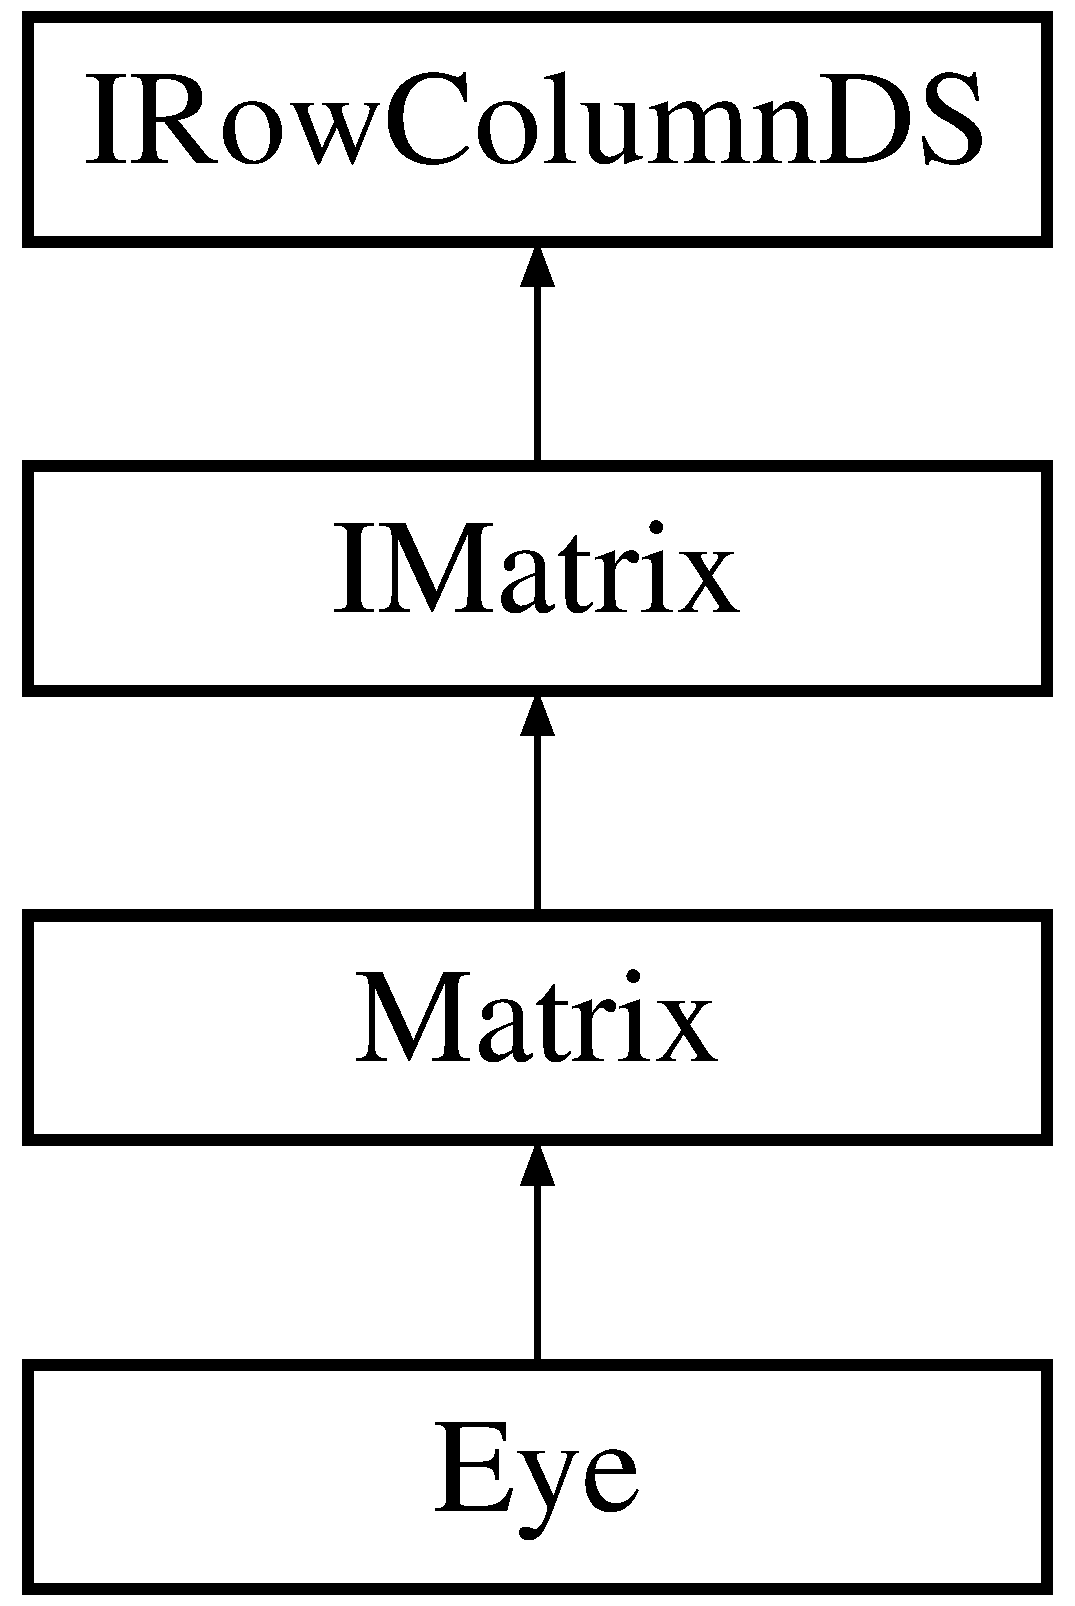
\includegraphics[height=4cm]{classIRowColumnDS}
\end{center}
\end{figure}
\subsection*{Public Member Functions}
\begin{DoxyCompactItemize}
\item 
\hypertarget{classIRowColumnDS_adb015e2f5cefbb187fbc150870c0e9c3}{
{\bfseries IRowColumnDS} (int M, int N, int nz, bool value)}
\label{classIRowColumnDS_adb015e2f5cefbb187fbc150870c0e9c3}

\item 
virtual \hyperlink{classIRowColumnDS_a70790b6b45416fde307ac8c7b456e005}{$\sim$IRowColumnDS} ()
\item 
\hypertarget{classIRowColumnDS_ac0d06d0f653f6eb9a2ac3d98a4d779aa}{
bool {\bfseries computeCCS} ()}
\label{classIRowColumnDS_ac0d06d0f653f6eb9a2ac3d98a4d779aa}

\item 
int \hyperlink{classIRowColumnDS_a29f440baacbd3f0cb4729ba9e868f2ae}{max} (int s, int t)
\item 
\hypertarget{classIRowColumnDS_af8420abed5c2b00e615120773a032dd0}{
int {\bfseries compress} ()}
\label{classIRowColumnDS_af8420abed5c2b00e615120773a032dd0}

\item 
bool \hyperlink{classIRowColumnDS_ab93c5ed2748d15f61ac047a033e0deca}{computeCRS} ()
\item 
void \hyperlink{classIRowColumnDS_a83fbd9be18ddd86a224ef172ca7eec6b}{setIndRowEntry} (int index, int entry)
\item 
\hypertarget{classIRowColumnDS_a4a259c7a9069d26fa51361d86cd66de5}{
void {\bfseries setIndColEntry} (int index, int entry)}
\label{classIRowColumnDS_a4a259c7a9069d26fa51361d86cd66de5}

\item 
\hypertarget{classIRowColumnDS_a90f101574c00ebb576b47e39b2ec42d7}{
void {\bfseries entry} (int row, int col, double value)}
\label{classIRowColumnDS_a90f101574c00ebb576b47e39b2ec42d7}

\item 
\hypertarget{classIRowColumnDS_a1f5253e46796967261bb4c70398351bb}{
void {\bfseries entry} (int row, int col)}
\label{classIRowColumnDS_a1f5253e46796967261bb4c70398351bb}

\item 
\hypertarget{classIRowColumnDS_aab9bc21c6d8fe6ae0ddc3d5cbdbf800c}{
int {\bfseries getIndRowEntry} (int index) const }
\label{classIRowColumnDS_aab9bc21c6d8fe6ae0ddc3d5cbdbf800c}

\item 
\hypertarget{classIRowColumnDS_ad02c91fece0cd06336b90435fdd7dcce}{
int {\bfseries getIndColEntry} (int index) const }
\label{classIRowColumnDS_ad02c91fece0cd06336b90435fdd7dcce}

\item 
\hypertarget{classIRowColumnDS_ac46184fffcad6c98eb6f68bc0727b5ce}{
int {\bfseries getJpntrEntry} (int index) const }
\label{classIRowColumnDS_ac46184fffcad6c98eb6f68bc0727b5ce}

\item 
\hypertarget{classIRowColumnDS_a1d7bbb5d66d9ab8ba993f64e168f0bc0}{
int {\bfseries getIpntrEntry} (int index) const }
\label{classIRowColumnDS_a1d7bbb5d66d9ab8ba993f64e168f0bc0}

\item 
\hypertarget{classIRowColumnDS_a7cd55fedcad51c74826a95db605376c8}{
double {\bfseries getX} (int index) const }
\label{classIRowColumnDS_a7cd55fedcad51c74826a95db605376c8}

\item 
int \hyperlink{classIRowColumnDS_a293b0ef58ea2e3e0ea7cf73fd32e17a8}{getRowMax} () const 
\item 
\hypertarget{classIRowColumnDS_adeaa359abf78b65c173fd7a56bb7552c}{
int {\bfseries getRowMin} () const }
\label{classIRowColumnDS_adeaa359abf78b65c173fd7a56bb7552c}

\item 
\hypertarget{classIRowColumnDS_a7a5bab6f0afe3b6c788cf6c5785d95fd}{
int {\bfseries getRowAvg} () const }
\label{classIRowColumnDS_a7a5bab6f0afe3b6c788cf6c5785d95fd}

\item 
\hypertarget{classIRowColumnDS_a800274902ac3ab78b5d5f4015a1f205b}{
int {\bfseries getColMax} () const }
\label{classIRowColumnDS_a800274902ac3ab78b5d5f4015a1f205b}

\item 
\hypertarget{classIRowColumnDS_a9c882be72a4f484403b6ed12579c3d3d}{
int {\bfseries getColMin} () const }
\label{classIRowColumnDS_a9c882be72a4f484403b6ed12579c3d3d}

\item 
\hypertarget{classIRowColumnDS_a1aad873a0882b519ed1c1d1a1bb01d02}{
int {\bfseries getColAvg} () const }
\label{classIRowColumnDS_a1aad873a0882b519ed1c1d1a1bb01d02}

\item 
\hypertarget{classIRowColumnDS_ab8f0eaadca8b7e1d43afe3dbd10209c6}{
int {\bfseries getNNZ} () const }
\label{classIRowColumnDS_ab8f0eaadca8b7e1d43afe3dbd10209c6}

\item 
\hypertarget{classIRowColumnDS_aa4914b0aeae6902ecfc4c88f6f0b39bf}{
int {\bfseries getM} () const }
\label{classIRowColumnDS_aa4914b0aeae6902ecfc4c88f6f0b39bf}

\item 
\hypertarget{classIRowColumnDS_a09a3057692b02533c04c2c7854f5ae00}{
int {\bfseries getN} () const }
\label{classIRowColumnDS_a09a3057692b02533c04c2c7854f5ae00}

\item 
int \hyperlink{classIRowColumnDS_ac7f6fa1d2c803ae267146dec1cb129c7}{min} (int s, int t)
\end{DoxyCompactItemize}
\subsection*{Protected Attributes}
\begin{DoxyCompactItemize}
\item 
\hypertarget{classIRowColumnDS_a38f103844515bad5dfb960c2d4549491}{
int {\bfseries M}}
\label{classIRowColumnDS_a38f103844515bad5dfb960c2d4549491}

\item 
\hypertarget{classIRowColumnDS_ac36383da33ced1c264cc4882d2cff1ec}{
int {\bfseries N}}
\label{classIRowColumnDS_ac36383da33ced1c264cc4882d2cff1ec}

\item 
\hypertarget{classIRowColumnDS_a6d46c23e5b2e11baf41560a971060f76}{
int {\bfseries nz}}
\label{classIRowColumnDS_a6d46c23e5b2e11baf41560a971060f76}

\item 
\hypertarget{classIRowColumnDS_ab427de42a8a4dd350b84de961e4a1a8a}{
int {\bfseries nnz}}
\label{classIRowColumnDS_ab427de42a8a4dd350b84de961e4a1a8a}

\item 
\hypertarget{classIRowColumnDS_a0618e0904dad8a46110f818a516756ad}{
int $\ast$ {\bfseries indRow}}
\label{classIRowColumnDS_a0618e0904dad8a46110f818a516756ad}

\item 
\hypertarget{classIRowColumnDS_a7093e763260e846f150cc5761d1acab9}{
int $\ast$ {\bfseries indCol}}
\label{classIRowColumnDS_a7093e763260e846f150cc5761d1acab9}

\item 
\hypertarget{classIRowColumnDS_a0291cfdb7c86a6d110b5418eadd5c54f}{
int $\ast$ {\bfseries jpntr}}
\label{classIRowColumnDS_a0291cfdb7c86a6d110b5418eadd5c54f}

\item 
\hypertarget{classIRowColumnDS_a7654945a2de4c55e54ebd987bedb3dcf}{
int $\ast$ {\bfseries ipntr}}
\label{classIRowColumnDS_a7654945a2de4c55e54ebd987bedb3dcf}

\item 
\hypertarget{classIRowColumnDS_a90be5162eb78e7cfcb66e6d65248e7fd}{
bool {\bfseries value}}
\label{classIRowColumnDS_a90be5162eb78e7cfcb66e6d65248e7fd}

\item 
\hypertarget{classIRowColumnDS_ab21b8c23bff745ef11651c0378c11006}{
double $\ast$ {\bfseries x}}
\label{classIRowColumnDS_ab21b8c23bff745ef11651c0378c11006}

\item 
\hypertarget{classIRowColumnDS_a4d0b55d922b890713a74813e1b1b745e}{
int {\bfseries entry\_\-index}}
\label{classIRowColumnDS_a4d0b55d922b890713a74813e1b1b745e}

\end{DoxyCompactItemize}


\subsection{Constructor \& Destructor Documentation}
\hypertarget{classIRowColumnDS_a70790b6b45416fde307ac8c7b456e005}{
\index{IRowColumnDS@{IRowColumnDS}!$\sim$IRowColumnDS@{$\sim$IRowColumnDS}}
\index{$\sim$IRowColumnDS@{$\sim$IRowColumnDS}!IRowColumnDS@{IRowColumnDS}}
\subsubsection[{$\sim$IRowColumnDS}]{\setlength{\rightskip}{0pt plus 5cm}IRowColumnDS::$\sim$IRowColumnDS ()\hspace{0.3cm}{\ttfamily  \mbox{[}virtual\mbox{]}}}}
\label{classIRowColumnDS_a70790b6b45416fde307ac8c7b456e005}
: Destructor  Date: 17.08.2009 

\subsection{Member Function Documentation}
\hypertarget{classIRowColumnDS_ab93c5ed2748d15f61ac047a033e0deca}{
\index{IRowColumnDS@{IRowColumnDS}!computeCRS@{computeCRS}}
\index{computeCRS@{computeCRS}!IRowColumnDS@{IRowColumnDS}}
\subsubsection[{computeCRS}]{\setlength{\rightskip}{0pt plus 5cm}bool IRowColumnDS::computeCRS ()}}
\label{classIRowColumnDS_ab93c5ed2748d15f61ac047a033e0deca}


$\ast$$\ast$$\ast$$\ast$$\ast$$\ast$$\ast$$\ast$$\ast$$\ast$

subroutine setr

given a column-\/oriented definition of the sparsity pattern of an M by N matrix a, this subroutine determines a row-\/oriented definition of the sparsity pattern of a.

on input the column-\/oriented definition is specified by the arrays indRow and jpntr. on output the row-\/oriented definition is specified by the arrays indCol and ipntr.

the subroutine statement is

subroutine setr(M,N,indRow,jpntr,indCol,ipntr,w)

where

M is a positive integer input variable set to the number of rows of a.

N is a positive integer input variable set to the number of columns of a.

indRow is an integer input array which contains the row indices for the non-\/zeroes in the matrix a.

jpntr is an integer input array of length N + 1 which specifies the locations of the row indices in indRow. the row indices for column j are

indRow\mbox{[}k\mbox{]}, k = jpntr\mbox{[}j\mbox{]},...,jpntr\mbox{[}j+1\mbox{]}-\/1.

note that jpntr\mbox{[}N+1\mbox{]}-\/1 is then the number of non-\/zero elements of the matrix a.

indCol is an integer output array which contains the column indices for the non-\/zeroes in the matrix a.

ipntr is an integer output array of length M + 1 which specifies the locations of the column indices in indCol. the column indices for row i are

indCol\mbox{[}k\mbox{]}, k = ipntr\mbox{[}i\mbox{]},...,ipntr\mbox{[}i+1\mbox{]}-\/1.

note that ipntr\mbox{[}1\mbox{]} is set to 1 and that ipntr\mbox{[}M+1\mbox{]}-\/1 is then the number of non-\/zero elements of the matrix a.

w is an integer work array of length M.

argonne national laboratory. minpack project. july 1983. thomas f. coleman, burton s. garbow, jorge j. more'\hypertarget{classIRowColumnDS_a293b0ef58ea2e3e0ea7cf73fd32e17a8}{
\index{IRowColumnDS@{IRowColumnDS}!getRowMax@{getRowMax}}
\index{getRowMax@{getRowMax}!IRowColumnDS@{IRowColumnDS}}
\subsubsection[{getRowMax}]{\setlength{\rightskip}{0pt plus 5cm}int IRowColumnDS::getRowMax () const}}
\label{classIRowColumnDS_a293b0ef58ea2e3e0ea7cf73fd32e17a8}
Statistical Methods \hypertarget{classIRowColumnDS_a29f440baacbd3f0cb4729ba9e868f2ae}{
\index{IRowColumnDS@{IRowColumnDS}!max@{max}}
\index{max@{max}!IRowColumnDS@{IRowColumnDS}}
\subsubsection[{max}]{\setlength{\rightskip}{0pt plus 5cm}int IRowColumnDS::max (int {\em s}, \/  int {\em t})}}
\label{classIRowColumnDS_a29f440baacbd3f0cb4729ba9e868f2ae}
Method max \hypertarget{classIRowColumnDS_ac7f6fa1d2c803ae267146dec1cb129c7}{
\index{IRowColumnDS@{IRowColumnDS}!min@{min}}
\index{min@{min}!IRowColumnDS@{IRowColumnDS}}
\subsubsection[{min}]{\setlength{\rightskip}{0pt plus 5cm}int IRowColumnDS::min (int {\em s}, \/  int {\em t})}}
\label{classIRowColumnDS_ac7f6fa1d2c803ae267146dec1cb129c7}
Method \hyperlink{classIRowColumnDS_ac7f6fa1d2c803ae267146dec1cb129c7}{min(int s, int t)} \hypertarget{classIRowColumnDS_a83fbd9be18ddd86a224ef172ca7eec6b}{
\index{IRowColumnDS@{IRowColumnDS}!setIndRowEntry@{setIndRowEntry}}
\index{setIndRowEntry@{setIndRowEntry}!IRowColumnDS@{IRowColumnDS}}
\subsubsection[{setIndRowEntry}]{\setlength{\rightskip}{0pt plus 5cm}void IRowColumnDS::setIndRowEntry (int {\em index}, \/  int {\em entry})}}
\label{classIRowColumnDS_a83fbd9be18ddd86a224ef172ca7eec6b}
Setter getter methods 

The documentation for this class was generated from the following files:\begin{DoxyCompactItemize}
\item 
src/IRowColumnDS.hh\item 
src/IRowColumnDS.cc\end{DoxyCompactItemize}

\hypertarget{structltint}{
\section{ltint Struct Reference}
\label{structltint}\index{ltint@{ltint}}
}
\subsection*{Public Member Functions}
\begin{DoxyCompactItemize}
\item 
\hypertarget{structltint_a66c11c4b7988f5144663a9d5120cda73}{
bool {\bfseries operator()} (const int i1, const int i2) const }
\label{structltint_a66c11c4b7988f5144663a9d5120cda73}

\end{DoxyCompactItemize}


The documentation for this struct was generated from the following file:\begin{DoxyCompactItemize}
\item 
src/NNZTag.hh\end{DoxyCompactItemize}

\hypertarget{classMatrix}{
\section{Matrix Class Reference}
\label{classMatrix}\index{Matrix@{Matrix}}
}


{\ttfamily \#include $<$Matrix.hh$>$}Inheritance diagram for Matrix::\begin{figure}[H]
\begin{center}
\leavevmode
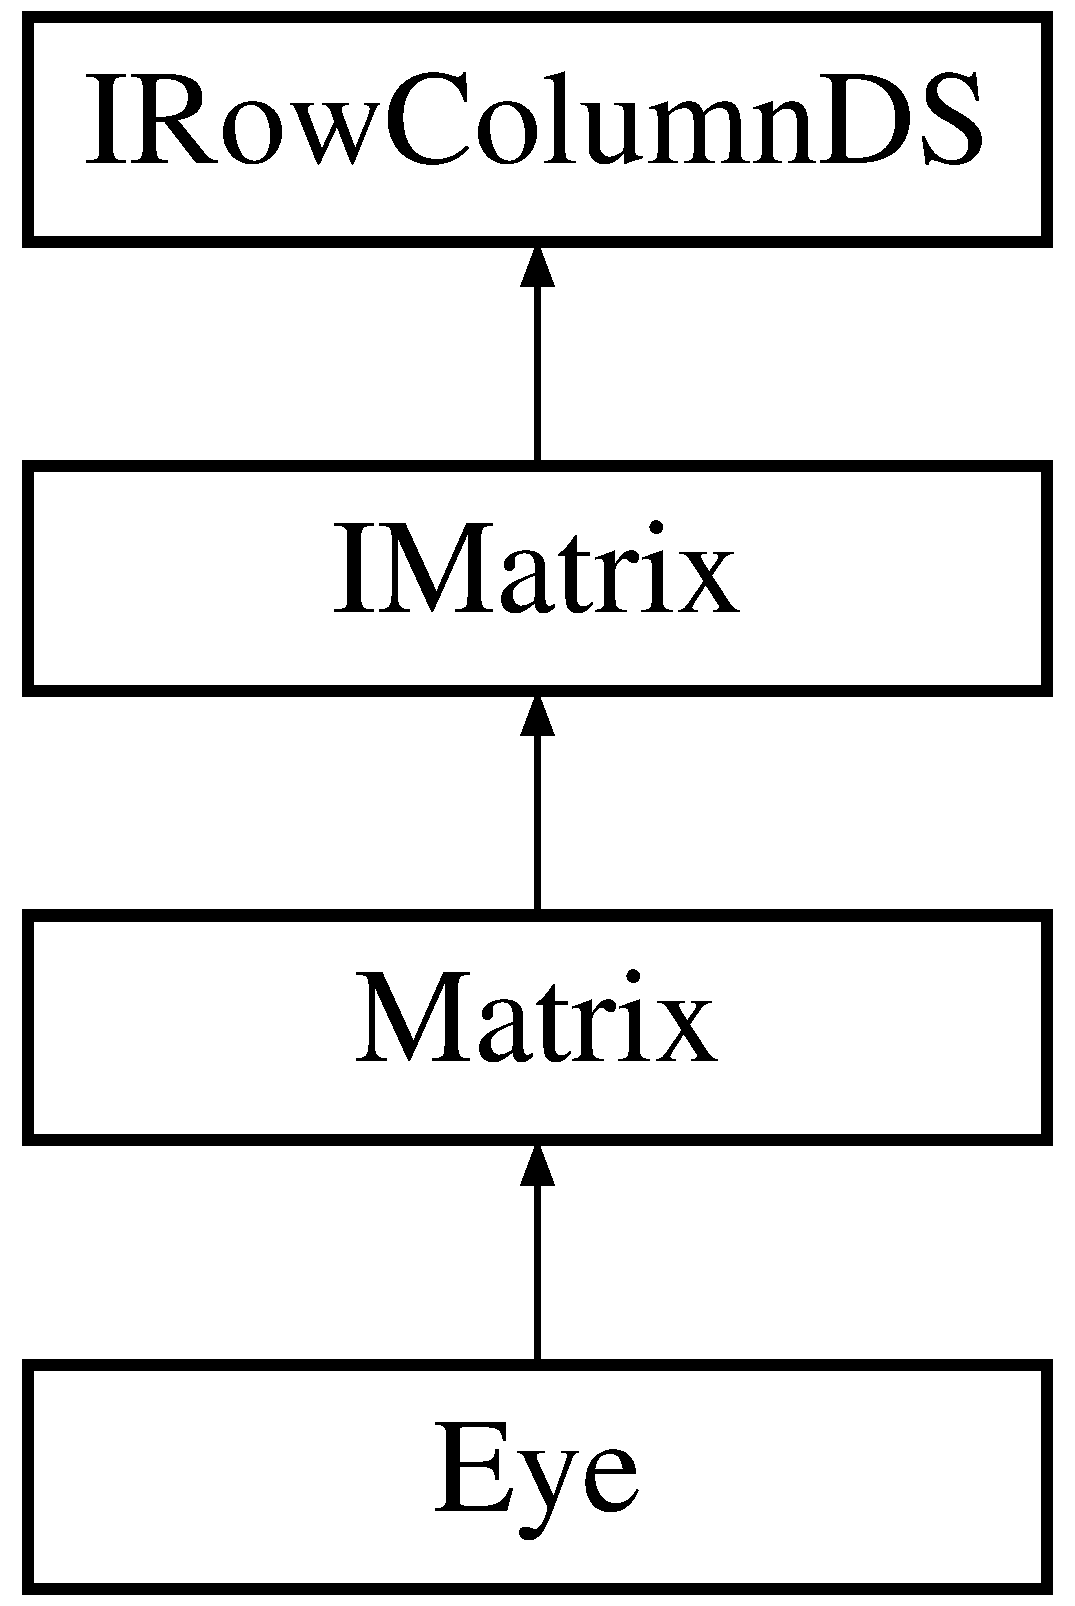
\includegraphics[height=4cm]{classMatrix}
\end{center}
\end{figure}
\subsection*{Public Member Functions}
\begin{DoxyCompactItemize}
\item 
\hyperlink{classMatrix_a9b1c3627f573d78a2f08623fdfef990f}{$\sim$Matrix} ()
\item 
\hyperlink{classMatrix_ae1ee0790f74689ac1ea9d6493e5ccd60}{Matrix} (int M, int N, int nz, bool value)
\item 
int \hyperlink{classMatrix_a7c1221aa40beeb82fdbacddcf86d58c9}{updateDegreesToUVertices} (int n, int ic, int u\_\-maxdeg, int $\ast$jpntr, int $\ast$indRow, int $\ast$ipntr, int $\ast$indCol, bool $\ast$f\_\-added, int $\ast$tag, int $\ast$f\_\-tag, int $\ast$u\_\-list, int $\ast$u\_\-head, int $\ast$u\_\-next, int $\ast$u\_\-previous, int $\ast$list, int $\ast$blackList, const int q)
\item 
bool \hyperlink{classMatrix_ac7e287f032e1296c51ce29704a0af704}{slo} (int $\ast$order)
\item 
bool \hyperlink{classMatrix_ab9bef57c1115e601cdeb493ecb381b82}{ido} (int $\ast$order)
\item 
bool \hyperlink{classMatrix_a24f9f912233b249ba1bb8e18eb979121}{lfo} (int $\ast$order)
\item 
bool \hyperlink{classMatrix_a6f6be59bfe0d4d5e1efae38f22174482}{computedegree} ()
\item 
int \hyperlink{classMatrix_a7ecfea6224fd953efa4a2add29307d0a}{greedycolor} (int $\ast$list, int $\ast$ngrp)
\item 
int \hyperlink{classMatrix_a55f7c0c85880d58823dd77aeefbd046c}{rlf} (int $\ast$ngrp)
\item 
int \hyperlink{classMatrix_a52e013055a3aef16751672815fc06600}{sdo} (int $\ast$ngrp)
\item 
\hypertarget{classMatrix_adbd4897b49ac42163ff50884a43499dc}{
\hyperlink{classMatrix}{Matrix} $\ast$ {\bfseries getSeedMatrix} (int $\ast$ngrp)}
\label{classMatrix_adbd4897b49ac42163ff50884a43499dc}

\item 
\hypertarget{classMatrix_aaa650ab5e57f0e1be15756184425794f}{
int {\bfseries getNumberOfColors} () const }
\label{classMatrix_aaa650ab5e57f0e1be15756184425794f}

\end{DoxyCompactItemize}


\subsection{Detailed Description}
\begin{Desc}
\item[\hyperlink{todo__todo000002}{Todo}]\end{Desc}


\subsection{Constructor \& Destructor Documentation}
\hypertarget{classMatrix_a9b1c3627f573d78a2f08623fdfef990f}{
\index{Matrix@{Matrix}!$\sim$Matrix@{$\sim$Matrix}}
\index{$\sim$Matrix@{$\sim$Matrix}!Matrix@{Matrix}}
\subsubsection[{$\sim$Matrix}]{\setlength{\rightskip}{0pt plus 5cm}Matrix::$\sim$Matrix ()}}
\label{classMatrix_a9b1c3627f573d78a2f08623fdfef990f}
Destructor \hypertarget{classMatrix_ae1ee0790f74689ac1ea9d6493e5ccd60}{
\index{Matrix@{Matrix}!Matrix@{Matrix}}
\index{Matrix@{Matrix}!Matrix@{Matrix}}
\subsubsection[{Matrix}]{\setlength{\rightskip}{0pt plus 5cm}Matrix::Matrix (int {\em M}, \/  int {\em N}, \/  int {\em nz}, \/  bool {\em value})}}
\label{classMatrix_ae1ee0790f74689ac1ea9d6493e5ccd60}
Constructor 

\subsection{Member Function Documentation}
\hypertarget{classMatrix_a6f6be59bfe0d4d5e1efae38f22174482}{
\index{Matrix@{Matrix}!computedegree@{computedegree}}
\index{computedegree@{computedegree}!Matrix@{Matrix}}
\subsubsection[{computedegree}]{\setlength{\rightskip}{0pt plus 5cm}bool Matrix::computedegree ()\hspace{0.3cm}{\ttfamily  \mbox{[}virtual\mbox{]}}}}
\label{classMatrix_a6f6be59bfe0d4d5e1efae38f22174482}
Purpose: Computes Degree sequence of the columns of a sparse matrix A (i.e. the vertices of the column intersection graph G(A) ).

Pre-\/condition: The matrix object is nonempty. Assumes that the computeCCS(), compress() and \hyperlink{classIRowColumnDS_ab93c5ed2748d15f61ac047a033e0deca}{computeCRS()} has been called prior calling this function, such that matrix object holds the sparsity information in Compressed Column and Compressed Row storage.

Post-\/condition: Degree information for the columns of matrix A ( graph G(A) ) is stored in the data member $<$id:ndeg$>$, an integer array of size n+1 such that if k = ndeg\mbox{[}j\mbox{]} then the column j has degree k, where j = 1,2, ...,n.

Return values: Returns true when the function is executed successfully, otherwise returns false. 

Implements \hyperlink{classIMatrix}{IMatrix}.\hypertarget{classMatrix_a7ecfea6224fd953efa4a2add29307d0a}{
\index{Matrix@{Matrix}!greedycolor@{greedycolor}}
\index{greedycolor@{greedycolor}!Matrix@{Matrix}}
\subsubsection[{greedycolor}]{\setlength{\rightskip}{0pt plus 5cm}int Matrix::greedycolor (int $\ast$ {\em order}, \/  int $\ast$ {\em color})\hspace{0.3cm}{\ttfamily  \mbox{[}virtual\mbox{]}}}}
\label{classMatrix_a7ecfea6224fd953efa4a2add29307d0a}
Purpose: Computes the greedy coloring of the columns of a sparse matrix A (i.e. the vertices of the column intersection graph G(A))

Pre-\/condition: The matrix object is nonempty. Assumes that an ordering has been provided in the in-\/parameter $<$id:order$>$ integer array of size n+1, such that order\mbox{[}1\mbox{]}...order\mbox{[}n\mbox{]} is a permutation of \{1,...,n\}

Post-\/condition: The greedy coloring of \hyperlink{classMatrix}{Matrix} A( graph G(A) ) is stored in the in-\/out-\/parameter $<$id:color$>$, an integer array of size n+1, such that if k = color\mbox{[}j\mbox{]} then the column j is colored with color k, j = 1,2,...,n

Parameters: in-\/parameter $<$id:order$>$, an integer pointer to an array of size n+1, containing a permutation of \{1,...,n\}. The integer array uses 1-\/based indexing.

in-\/out-\/parameter $<$id:color$>$, an integer pointer to an array of size n+1, it stores the color values of the columns in successful completion.The integer array uses 1-\/based indexing.

Return values: Returns the number of colors if succeeds, otherwise returns 0(zero). 

Implements \hyperlink{classIMatrix}{IMatrix}.\hypertarget{classMatrix_ab9bef57c1115e601cdeb493ecb381b82}{
\index{Matrix@{Matrix}!ido@{ido}}
\index{ido@{ido}!Matrix@{Matrix}}
\subsubsection[{ido}]{\setlength{\rightskip}{0pt plus 5cm}bool Matrix::ido (int $\ast$ {\em order})\hspace{0.3cm}{\ttfamily  \mbox{[}virtual\mbox{]}}}}
\label{classMatrix_ab9bef57c1115e601cdeb493ecb381b82}
Method \hyperlink{classMatrix_ab9bef57c1115e601cdeb493ecb381b82}{ido()}

Purpose: Computes Incidence-\/Degree Ordering (IDO) of the columns of a sparse matrix A (i.e. the vertices of the column intersection graph G(A) )

Pre-\/condition: The matrix object is nonempty. Assumes that the degree of of the columns have already been computed in the data member $<$id:ndeg$>$ integer array of size n+1 using computeDegree() method.

Post-\/condition: The IDO ordering of matrix A ( graph G(A) ) is stored in the out-\/parameter $<$id:order$>$, an integer array of size n+1 such that if k = order\mbox{[}j\mbox{]} then the column j is the k-\/th element, k = 1,2, ..., n, in the IDO ordering, and j = 1,2, ..., n.

Parameters: out-\/parameter $<$id:order$>$, an integer pointer to an array of size n+1. The array will contain the ordering information when the function normally returns.

Return values: Returns true when the function is executed successfully, otherwise returns false. 

Implements \hyperlink{classIMatrix_a8e0f3a1062786b6a20548e847de1109b}{IMatrix}.\hypertarget{classMatrix_a24f9f912233b249ba1bb8e18eb979121}{
\index{Matrix@{Matrix}!lfo@{lfo}}
\index{lfo@{lfo}!Matrix@{Matrix}}
\subsubsection[{lfo}]{\setlength{\rightskip}{0pt plus 5cm}bool Matrix::lfo (int $\ast$ {\em order})\hspace{0.3cm}{\ttfamily  \mbox{[}virtual\mbox{]}}}}
\label{classMatrix_a24f9f912233b249ba1bb8e18eb979121}
Purpose: Computes Largest-\/First Ordering (LFO) of the columns of a sparse matrix A (i.e. the vertices of the column intersection graph G(A) )

Pre-\/condition: The matrix object is nonempty. Assumes that the degree of of the columns have already been computed in the data member $<$id:ndeg$>$ integer array of size n+1 using computeDegree() method.

Post-\/condition: The LFO ordering of matrix A ( graph G(A) ) is stored in the out-\/parameter $<$id:order$>$, an integer array of size n+1 such that if k = order\mbox{[}j\mbox{]} then the column j is the k-\/th element, k = 1,2, ..., n, in the LFO ordering, and j = 1,2, ..., n.

Parameters: out-\/parameter $<$id:order$>$, an integer pointer to an array of size n+1. The array will contain the ordering information when the function normally returns.

Return values: Returns true when the function is executed successfully, otherwise returns false. 

Implements \hyperlink{classIMatrix}{IMatrix}.\hypertarget{classMatrix_a55f7c0c85880d58823dd77aeefbd046c}{
\index{Matrix@{Matrix}!rlf@{rlf}}
\index{rlf@{rlf}!Matrix@{Matrix}}
\subsubsection[{rlf}]{\setlength{\rightskip}{0pt plus 5cm}int Matrix::rlf (int $\ast$ {\em color})\hspace{0.3cm}{\ttfamily  \mbox{[}virtual\mbox{]}}}}
\label{classMatrix_a55f7c0c85880d58823dd77aeefbd046c}
Purpose: Computes Recursive Largest-\/First coloring (\hyperlink{classRLF}{RLF}) of the columns of a sparse matrix A (i.e. the vertices of the column intersection graph G(A) )

Pre-\/condition: The matrix object is nonempty. Assumes that the degree of of the columns have already been computed in the data member $<$id:ndeg$>$ integer array of size n+1 using computeDegree() method.

Post-\/condition: \hyperlink{classRLF}{RLF} coloring of \hyperlink{classMatrix}{Matrix} A(graph G(A)) is stored in the in-\/out-\/parameter $<$id:color$>$, an integer array of size n+1, such that if k = color\mbox{[}j\mbox{]} then the column j is colored with color k, j = 1,2,...,n

Parameters: out-\/parameter $<$id:color$>$, an integer pointer to an array of size n+1. The array will contain the color values of the columns in successful completion. The integer array uses 1-\/based indexing.

Return values: Returns the number of colors if succeeds, otherwise returns 0(zero). 

Implements \hyperlink{classIMatrix}{IMatrix}.\hypertarget{classMatrix_a52e013055a3aef16751672815fc06600}{
\index{Matrix@{Matrix}!sdo@{sdo}}
\index{sdo@{sdo}!Matrix@{Matrix}}
\subsubsection[{sdo}]{\setlength{\rightskip}{0pt plus 5cm}int Matrix::sdo (int $\ast$ {\em color})}}
\label{classMatrix_a52e013055a3aef16751672815fc06600}
: This method is called when we move a vertex from set V' to set U. This method has a complexity of \{\}

: This method is called when we move a vertex from set V' to set U. This method has a complexity of \{\} Purpose: Computes Saturation-\/Degree Coloring(or Ordering) (SDO) of the columns of a sparse matrix A (i.e. the vertices of the column intersection graph G(A) )

Pre-\/condition: The matrix object is nonempty. Assumes that the degree of of the columns have already been computed in the data member $<$id:ndeg$>$ integer array of size n+1 using computeDegree() method.

Post-\/condition: SDO coloring of \hyperlink{classMatrix}{Matrix} A(graph G(A)) is stored in the in-\/out-\/parameter $<$id:color$>$, an integer array of size n+1, such that if k = color\mbox{[}j\mbox{]} then the column j is colored with color k, j = 1,2,...,n

Parameters: out-\/parameter $<$id:color$>$, an integer pointer to an array of size n+1. The array will contain the color values of the columns in successful completion. The integer array uses 1-\/based indexing.

Return values: Returns the number of colors if succeeds, otherwise returns 0(zero). \hypertarget{classMatrix_ac7e287f032e1296c51ce29704a0af704}{
\index{Matrix@{Matrix}!slo@{slo}}
\index{slo@{slo}!Matrix@{Matrix}}
\subsubsection[{slo}]{\setlength{\rightskip}{0pt plus 5cm}bool Matrix::slo (int $\ast$ {\em list})\hspace{0.3cm}{\ttfamily  \mbox{[}virtual\mbox{]}}}}
\label{classMatrix_ac7e287f032e1296c51ce29704a0af704}
Purpose: Computes Smallest-\/Last Ordering (SLO) of the columns of a sparse matrix A (i.e. the vertices of the column intersection graph G(A) )

Pre-\/condition: The matrix object is nonempty. Assumes that the degree of of the columns have already been computed in the data member $<$id:ndeg$>$ integer array of size n+1 using computeDegree() method.

Post-\/condition: The SLO ordering of matrix A ( graph G(A) ) is stored in the out-\/parameter $<$id:list$>$, an integer array of size n+1 such that if k = list\mbox{[}j\mbox{]} then the column j is the k-\/th element, k = 1,2, ..., n, in the SLO ordering, and j = 1,2, ..., n.

Parameters: out-\/parameter $<$id:list$>$, an integer pointer to an array of size n+1. The array will contain the ordering information when the function normally returns.

Return values: Returns true when the function is executed successfully, otherwise returns false. 

Implements \hyperlink{classIMatrix_ad6d689b7a38120b6463f1965915f7163}{IMatrix}.\hypertarget{classMatrix_a7c1221aa40beeb82fdbacddcf86d58c9}{
\index{Matrix@{Matrix}!updateDegreesToUVertices@{updateDegreesToUVertices}}
\index{updateDegreesToUVertices@{updateDegreesToUVertices}!Matrix@{Matrix}}
\subsubsection[{updateDegreesToUVertices}]{\setlength{\rightskip}{0pt plus 5cm}int Matrix::updateDegreesToUVertices (int {\em n}, \/  int {\em ic}, \/  int {\em u\_\-maxdeg}, \/  int $\ast$ {\em jpntr}, \/  int $\ast$ {\em indRow}, \/  int $\ast$ {\em ipntr}, \/  int $\ast$ {\em indCol}, \/  bool $\ast$ {\em f\_\-added}, \/  int $\ast$ {\em tag}, \/  int $\ast$ {\em f\_\-tag}, \/  int $\ast$ {\em u\_\-list}, \/  int $\ast$ {\em u\_\-head}, \/  int $\ast$ {\em u\_\-next}, \/  int $\ast$ {\em u\_\-previous}, \/  int $\ast$ {\em list}, \/  int $\ast$ {\em blackList}, \/  const int {\em q})}}
\label{classMatrix_a7c1221aa40beeb82fdbacddcf86d58c9}


Update the pointers to the current degree u\_\-lists.

The documentation for this class was generated from the following files:\begin{DoxyCompactItemize}
\item 
src/Matrix.hh\item 
src/Matrix.cpp\end{DoxyCompactItemize}

\hypertarget{classDSJM_1_1MemoryError}{
\section{DSJM::MemoryError Class Reference}
\label{classDSJM_1_1MemoryError}\index{DSJM::MemoryError@{DSJM::MemoryError}}
}


The documentation for this class was generated from the following file:\begin{DoxyCompactItemize}
\item 
src/Utility.h\end{DoxyCompactItemize}

\hypertarget{classNNZTag}{
\section{NNZTag Class Reference}
\label{classNNZTag}\index{NNZTag@{NNZTag}}
}
\subsection*{Public Member Functions}
\begin{DoxyCompactItemize}
\item 
\hyperlink{classNNZTag_ad06478eaa480ac4b33390782efa7d8b9}{NNZTag} (int m, int n)
\item 
virtual \hyperlink{classNNZTag_ac7a5b8cb937bc062d605a37dbcee62be}{$\sim$NNZTag} ()
\item 
int \hyperlink{classNNZTag_ab93956ff16797fdb7c1e55eeb2e3549c}{getValue} (int row, int column)
\item 
void \hyperlink{classNNZTag_a88006fcd4a4d2386c16f196c2cc2b08c}{setValue} (int row, int column, int value)
\end{DoxyCompactItemize}


\subsection{Constructor \& Destructor Documentation}
\hypertarget{classNNZTag_ad06478eaa480ac4b33390782efa7d8b9}{
\index{NNZTag@{NNZTag}!NNZTag@{NNZTag}}
\index{NNZTag@{NNZTag}!NNZTag@{NNZTag}}
\subsubsection[{NNZTag}]{\setlength{\rightskip}{0pt plus 5cm}NNZTag::NNZTag (int {\em \_\-M}, \/  int {\em \_\-N})}}
\label{classNNZTag_ad06478eaa480ac4b33390782efa7d8b9}
: Constructor  Date: 09.08.2009 \hypertarget{classNNZTag_ac7a5b8cb937bc062d605a37dbcee62be}{
\index{NNZTag@{NNZTag}!$\sim$NNZTag@{$\sim$NNZTag}}
\index{$\sim$NNZTag@{$\sim$NNZTag}!NNZTag@{NNZTag}}
\subsubsection[{$\sim$NNZTag}]{\setlength{\rightskip}{0pt plus 5cm}NNZTag::$\sim$NNZTag ()\hspace{0.3cm}{\ttfamily  \mbox{[}virtual\mbox{]}}}}
\label{classNNZTag_ac7a5b8cb937bc062d605a37dbcee62be}
: Destructor  Date: 09.08.2009 

\subsection{Member Function Documentation}
\hypertarget{classNNZTag_ab93956ff16797fdb7c1e55eeb2e3549c}{
\index{NNZTag@{NNZTag}!getValue@{getValue}}
\index{getValue@{getValue}!NNZTag@{NNZTag}}
\subsubsection[{getValue}]{\setlength{\rightskip}{0pt plus 5cm}int NNZTag::getValue (int {\em row}, \/  int {\em column})}}
\label{classNNZTag_ab93956ff16797fdb7c1e55eeb2e3549c}
: Getter Function  Date: 09.08.2009 \hypertarget{classNNZTag_a88006fcd4a4d2386c16f196c2cc2b08c}{
\index{NNZTag@{NNZTag}!setValue@{setValue}}
\index{setValue@{setValue}!NNZTag@{NNZTag}}
\subsubsection[{setValue}]{\setlength{\rightskip}{0pt plus 5cm}void NNZTag::setValue (int {\em row}, \/  int {\em column}, \/  int {\em value})}}
\label{classNNZTag_a88006fcd4a4d2386c16f196c2cc2b08c}
: Setter Method  Date: 09.08.2009 

The documentation for this class was generated from the following files:\begin{DoxyCompactItemize}
\item 
src/NNZTag.hh\item 
src/NNZTag.cc\end{DoxyCompactItemize}

\hypertarget{classResult}{
\section{Result Class Reference}
\label{classResult}\index{Result@{Result}}
}
\subsection*{Public Member Functions}
\begin{DoxyCompactItemize}
\item 
\hypertarget{classResult_a5235cad2b14b69ee69405a2c425ac58e}{
void {\bfseries printInfo} ()}
\label{classResult_a5235cad2b14b69ee69405a2c425ac58e}

\item 
\hypertarget{classResult_a35d12d80d3226b04b521b4935f306eea}{
void {\bfseries printMatrixInfo} ()}
\label{classResult_a35d12d80d3226b04b521b4935f306eea}

\item 
\hypertarget{classResult_adbd8c390724b16f7b88da3036fa26307}{
void {\bfseries printResult} ()}
\label{classResult_adbd8c390724b16f7b88da3036fa26307}

\end{DoxyCompactItemize}
\subsection*{Public Attributes}
\begin{DoxyCompactItemize}
\item 
\hypertarget{classResult_ad90fd8872d7c9429f28275ed708496cd}{
int {\bfseries matrix\_\-M}}
\label{classResult_ad90fd8872d7c9429f28275ed708496cd}

\item 
\hypertarget{classResult_a6dfcad37c4f4f6bd3a865d50e8e0130b}{
int {\bfseries matrix\_\-N}}
\label{classResult_a6dfcad37c4f4f6bd3a865d50e8e0130b}

\item 
\hypertarget{classResult_a30928aeb2ac524d5f60f307ca058450e}{
int {\bfseries matrix\_\-NNZ}}
\label{classResult_a30928aeb2ac524d5f60f307ca058450e}

\item 
\hypertarget{classResult_af035e8ca1f67ddafa5afe98fd73058a4}{
int {\bfseries rowMax}}
\label{classResult_af035e8ca1f67ddafa5afe98fd73058a4}

\item 
\hypertarget{classResult_ac7d51cf1315500e193fc02177dd9ae19}{
int {\bfseries rowAvg}}
\label{classResult_ac7d51cf1315500e193fc02177dd9ae19}

\item 
\hypertarget{classResult_acceb25d44896f0828d8df541e5e34136}{
int {\bfseries rowMin}}
\label{classResult_acceb25d44896f0828d8df541e5e34136}

\item 
\hypertarget{classResult_a0de92f0fd2f97204895890d28c66d191}{
int {\bfseries colMax}}
\label{classResult_a0de92f0fd2f97204895890d28c66d191}

\item 
\hypertarget{classResult_aa97ebcdac8e1b7f661ef4814aff95441}{
int {\bfseries colAvg}}
\label{classResult_aa97ebcdac8e1b7f661ef4814aff95441}

\item 
\hypertarget{classResult_a4d874b6ce4aad1088ed107fe5068d381}{
int {\bfseries colMin}}
\label{classResult_a4d874b6ce4aad1088ed107fe5068d381}

\item 
\hypertarget{classResult_af6746447e5952d059a22f8610b994122}{
bool {\bfseries is\_\-Cseg}}
\label{classResult_af6746447e5952d059a22f8610b994122}

\item 
\hypertarget{classResult_a6d4c85096335bd8ced0213269bee9a8b}{
\hyperlink{classConfiguration}{Configuration} $\ast$ {\bfseries configuration}}
\label{classResult_a6d4c85096335bd8ced0213269bee9a8b}

\item 
\hypertarget{classResult_a3d24ec89902e66df00154915fc40f24b}{
CLI::ordering\_\-method {\bfseries method}}
\label{classResult_a3d24ec89902e66df00154915fc40f24b}

\item 
\hypertarget{classResult_ab3fb3b1917106d9d8b5a41c4bd62fae6}{
int {\bfseries totalColors}}
\label{classResult_ab3fb3b1917106d9d8b5a41c4bd62fae6}

\item 
\hypertarget{classResult_a67815d21a6795ee76113c6894c1a097d}{
double {\bfseries ordering\_\-time}}
\label{classResult_a67815d21a6795ee76113c6894c1a097d}

\item 
\hypertarget{classResult_ae70ae8efb6a22efc0f69ca93d2d5f8e9}{
double {\bfseries coloring\_\-time}}
\label{classResult_ae70ae8efb6a22efc0f69ca93d2d5f8e9}

\item 
\hypertarget{classResult_a5670324c2b7ea794e4ebc68035511f6e}{
string {\bfseries inputFile}}
\label{classResult_a5670324c2b7ea794e4ebc68035511f6e}

\item 
\hypertarget{classResult_ad32c047d13f46b4bf1c004e6fb1edb69}{
string {\bfseries partitionFile}}
\label{classResult_ad32c047d13f46b4bf1c004e6fb1edb69}

\end{DoxyCompactItemize}


The documentation for this class was generated from the following file:\begin{DoxyCompactItemize}
\item 
src/Result.hh\end{DoxyCompactItemize}

\hypertarget{classRLF}{
\section{RLF Class Reference}
\label{classRLF}\index{RLF@{RLF}}
}
\subsection*{Public Member Functions}
\begin{DoxyCompactItemize}
\item 
\hypertarget{classRLF_a5d1fd0749544610d7573ab3cb2fecf1a}{
{\footnotesize template$<$typename PreviousOrderingMethod $>$ }\\{\bfseries RLF} (int M\_\-, int N\_\-, int $\ast$ndeg\_\-, int $\ast$jpntr\_\-, int $\ast$indRow\_\-, int $\ast$ipntr\_\-, int $\ast$indCol\_\-, int $\ast$list\_\-, int $\ast$ngrp\_\-, int maxBucket\_\-, PreviousOrderingMethod \&previousOrderingMethod, int howMany\_\-)}
\label{classRLF_a5d1fd0749544610d7573ab3cb2fecf1a}

\item 
int \hyperlink{classRLF_a327af9b44d25f836502b0184a98e673d}{work} ()
\item 
\hypertarget{classRLF_acde1c9e75affce9be79796b065b71d29}{
int {\bfseries getDeg} (int jcol)}
\label{classRLF_acde1c9e75affce9be79796b065b71d29}

\item 
\hypertarget{classRLF_acfd8a03e49e1122927b297de5d2e5aca}{
int {\bfseries getNumOrd} ()}
\label{classRLF_acfd8a03e49e1122927b297de5d2e5aca}

\item 
\hypertarget{classRLF_a188650f31e55c11f0dbbc2fc53697ec6}{
void {\bfseries tagit} (int jcol)}
\label{classRLF_a188650f31e55c11f0dbbc2fc53697ec6}

\item 
\hypertarget{classRLF_a1aef590b0a66b214e48378c9b8618d6f}{
void {\bfseries tagit} (int jcol, int value)}
\label{classRLF_a1aef590b0a66b214e48378c9b8618d6f}

\item 
\hypertarget{classRLF_a5c45cecd023ceff0279a6155b26fc0ce}{
void {\bfseries untagit} (int jcol)}
\label{classRLF_a5c45cecd023ceff0279a6155b26fc0ce}

\item 
\hypertarget{classRLF_aefb3a2f842f26794c5f9dff02dd79dd7}{
bool {\bfseries isTagged} (int jcol)}
\label{classRLF_aefb3a2f842f26794c5f9dff02dd79dd7}

\item 
\hypertarget{classRLF_a83954f50be5700233af332d0e3a36ca4}{
int {\bfseries getNumOrd} () const }
\label{classRLF_a83954f50be5700233af332d0e3a36ca4}

\end{DoxyCompactItemize}
\subsection*{Static Public Member Functions}
\begin{DoxyCompactItemize}
\item 
\hypertarget{classRLF_a601cf7fff1ba0d4725723739ac4ca7a4}{
{\footnotesize template$<$typename T\_\-PriorityQueue , typename Tag $>$ }\\static int {\bfseries pq\_\-updateDegreesToUVertices} (int n, int jcol, int maxdeg, int $\ast$jpntr, int $\ast$indRow, int $\ast$ipntr, int $\ast$indCol, bool $\ast$inU, Tag \&tag, int $\ast$u\_\-tag, T\_\-PriorityQueue \&u\_\-queue, int $\ast$blackList, const int q)}
\label{classRLF_a601cf7fff1ba0d4725723739ac4ca7a4}

\item 
\hypertarget{classRLF_a03f1d1159fba88ffcf071ccf3b7e26b2}{
{\footnotesize template$<$typename T\_\-PriorityQueue , typename Tag $>$ }\\static void {\bfseries pq\_\-initializeDegreesToUVertices} (int n, Tag \&tag, T\_\-PriorityQueue \&u\_\-queue, bool $\ast$inU, int $\ast$u\_\-tag)}
\label{classRLF_a03f1d1159fba88ffcf071ccf3b7e26b2}

\end{DoxyCompactItemize}
\subsection*{Public Attributes}
\begin{DoxyCompactItemize}
\item 
\hypertarget{classRLF_a281dd488844b24d24d5bc86a1e9c04ab}{
const OrderingMethod::ordering\_\-direction {\bfseries ord\_\-direction}}
\label{classRLF_a281dd488844b24d24d5bc86a1e9c04ab}

\end{DoxyCompactItemize}


\subsection{Member Function Documentation}
\hypertarget{classRLF_a327af9b44d25f836502b0184a98e673d}{
\index{RLF@{RLF}!work@{work}}
\index{work@{work}!RLF@{RLF}}
\subsubsection[{work}]{\setlength{\rightskip}{0pt plus 5cm}int RLF::work ()\hspace{0.3cm}{\ttfamily  \mbox{[}inline\mbox{]}}}}
\label{classRLF_a327af9b44d25f836502b0184a98e673d}


Choose a column jcol of maximal degree mindeg.

Choose a column jcol that has maximal degree in set U.

Tag the column, as it has been colored.

Find All Columns adjacent to column jcol. Determine all positions (ir,jcol) which correspond to non-\/zeroes in the matrix.

For each row ir, determine all positions (ir,ic) which correspond to non-\/zeroes in the matrix.

Array tag marks columns whch are adjacent to column jcol

We found the solution

We are supposed to initialize V, U

The documentation for this class was generated from the following file:\begin{DoxyCompactItemize}
\item 
src/RLF.hh\end{DoxyCompactItemize}

\hypertarget{classRunningTimeInfo}{
\section{RunningTimeInfo Class Reference}
\label{classRunningTimeInfo}\index{RunningTimeInfo@{RunningTimeInfo}}
}
\subsection*{Public Member Functions}
\begin{DoxyCompactItemize}
\item 
\hypertarget{classRunningTimeInfo_a05cd38673e446b2e6c19fa046cc922eb}{
{\bfseries RunningTimeInfo} (int c, double o\_\-t, double c\_\-t, int $\ast$grp)}
\label{classRunningTimeInfo_a05cd38673e446b2e6c19fa046cc922eb}

\end{DoxyCompactItemize}
\subsection*{Public Attributes}
\begin{DoxyCompactItemize}
\item 
\hypertarget{classRunningTimeInfo_a00617e5bffda55064c3f99a200c9556d}{
int {\bfseries color}}
\label{classRunningTimeInfo_a00617e5bffda55064c3f99a200c9556d}

\item 
\hypertarget{classRunningTimeInfo_aa53698235638e25f25129fd238844a37}{
double {\bfseries ordering\_\-time}}
\label{classRunningTimeInfo_aa53698235638e25f25129fd238844a37}

\item 
\hypertarget{classRunningTimeInfo_a708e9f967d88e666053ce48b40f5a771}{
double {\bfseries coloring\_\-time}}
\label{classRunningTimeInfo_a708e9f967d88e666053ce48b40f5a771}

\item 
\hypertarget{classRunningTimeInfo_a0d549de50aff87a8c992839b28ec6491}{
int $\ast$ {\bfseries ngrp}}
\label{classRunningTimeInfo_a0d549de50aff87a8c992839b28ec6491}

\end{DoxyCompactItemize}


The documentation for this class was generated from the following file:\begin{DoxyCompactItemize}
\item 
examples/driver.cc\end{DoxyCompactItemize}

\hypertarget{classStructuredJacobian}{
\section{StructuredJacobian Class Reference}
\label{classStructuredJacobian}\index{StructuredJacobian@{StructuredJacobian}}
}
\subsection*{Public Member Functions}
\begin{DoxyCompactItemize}
\item 
\hypertarget{classStructuredJacobian_a0216141d95994988564f1790fa383b4d}{
{\bfseries StructuredJacobian} (int n)}
\label{classStructuredJacobian_a0216141d95994988564f1790fa383b4d}

\item 
\hypertarget{classStructuredJacobian_a5779429aac9b8779b356ef28b983b118}{
auto\_\-ptr$<$ Sparsity $>$ {\bfseries getSparsityPattern} ()}
\label{classStructuredJacobian_a5779429aac9b8779b356ef28b983b118}

\item 
\hypertarget{classStructuredJacobian_a9ff4b938253fcd4699eaba35ca7095dc}{
auto\_\-ptr$<$ vector$<$ double $>$ $>$ {\bfseries eval} (const vector$<$ double $>$ \&x)}
\label{classStructuredJacobian_a9ff4b938253fcd4699eaba35ca7095dc}

\item 
\hypertarget{classStructuredJacobian_a934845213ab9d431deb7fdffb18ea2ee}{
\hyperlink{classMatrix}{Matrix} $\ast$ {\bfseries derivative} (const vector$<$ double $>$ \&x)}
\label{classStructuredJacobian_a934845213ab9d431deb7fdffb18ea2ee}

\item 
\hypertarget{classStructuredJacobian_ac7bb7523ef0c55143901e6b697cc8e30}{
double $\ast$ {\bfseries arrayderivative} (const vector$<$ double $>$ \&x)}
\label{classStructuredJacobian_ac7bb7523ef0c55143901e6b697cc8e30}

\item 
\hypertarget{classStructuredJacobian_a7b3fc3204d863ba9a513df9de0184cd7}{
int {\bfseries getNzmax} (const int n) const }
\label{classStructuredJacobian_a7b3fc3204d863ba9a513df9de0184cd7}

\end{DoxyCompactItemize}
\subsection*{Public Attributes}
\begin{DoxyCompactItemize}
\item 
\hypertarget{classStructuredJacobian_a34e166b7cf8761257f5c87b0cbfd0534}{
int {\bfseries n}}
\label{classStructuredJacobian_a34e166b7cf8761257f5c87b0cbfd0534}

\item 
\hypertarget{classStructuredJacobian_a60ded81d1f6e64c9d8f8b374ce625927}{
int {\bfseries m}}
\label{classStructuredJacobian_a60ded81d1f6e64c9d8f8b374ce625927}

\end{DoxyCompactItemize}


The documentation for this class was generated from the following files:\begin{DoxyCompactItemize}
\item 
examples/StructuredJacobian.hh\item 
examples/StructuredJacobian.cc\end{DoxyCompactItemize}

\hypertarget{classColPack_1_1Timer}{
\section{ColPack::Timer Class Reference}
\label{classColPack_1_1Timer}\index{ColPack::Timer@{ColPack::Timer}}
}


class \hyperlink{classColPack_1_1Timer}{Timer} in \hyperlink{}{group4}.  


{\ttfamily \#include $<$Timer.h$>$}\subsection*{Public Member Functions}
\begin{DoxyCompactItemize}
\item 
\hypertarget{classColPack_1_1Timer_a2ee878c906acc649e315741783729748}{
void {\bfseries Start} ()}
\label{classColPack_1_1Timer_a2ee878c906acc649e315741783729748}

\item 
\hypertarget{classColPack_1_1Timer_aee44f24596bbc8bfeea07eb85b699f79}{
void {\bfseries Stop} ()}
\label{classColPack_1_1Timer_aee44f24596bbc8bfeea07eb85b699f79}

\item 
\hypertarget{classColPack_1_1Timer_afa9cdbc07f53e5b09b5b1101930b05ec}{
double {\bfseries GetWallTime} ()}
\label{classColPack_1_1Timer_afa9cdbc07f53e5b09b5b1101930b05ec}

\item 
\hypertarget{classColPack_1_1Timer_a3ca3b7a0736317bec308c1d9db702dd0}{
double {\bfseries GetProcessorTime} ()}
\label{classColPack_1_1Timer_a3ca3b7a0736317bec308c1d9db702dd0}

\item 
\hypertarget{classColPack_1_1Timer_aeb1ba675cefe25bbea493ce25af1e67c}{
double {\bfseries GetUserProcessorTime} ()}
\label{classColPack_1_1Timer_aeb1ba675cefe25bbea493ce25af1e67c}

\item 
\hypertarget{classColPack_1_1Timer_a396a4839280ad5e4f06da4b7d1ee07f5}{
double {\bfseries GetSystemProcessorTime} ()}
\label{classColPack_1_1Timer_a396a4839280ad5e4f06da4b7d1ee07f5}

\end{DoxyCompactItemize}


\subsection{Detailed Description}
class \hyperlink{classColPack_1_1Timer}{Timer} in \hyperlink{}{group4}. The timer class is the only class in ColPack which has an optional dependency on the operating system. It offers both system independent C++ timer based on ctime.h or linux/unix dependent timer based on sys/times.h. The sytem independent timer only gives wall clock time while linux/unix dependent timer gives wall, processor, user and system times. 

The documentation for this class was generated from the following files:\begin{DoxyCompactItemize}
\item 
src/Timer.h\item 
src/Timer.cpp\end{DoxyCompactItemize}

\printindex
\end{document}
